\begin{figure}[htbp]
    \centering
    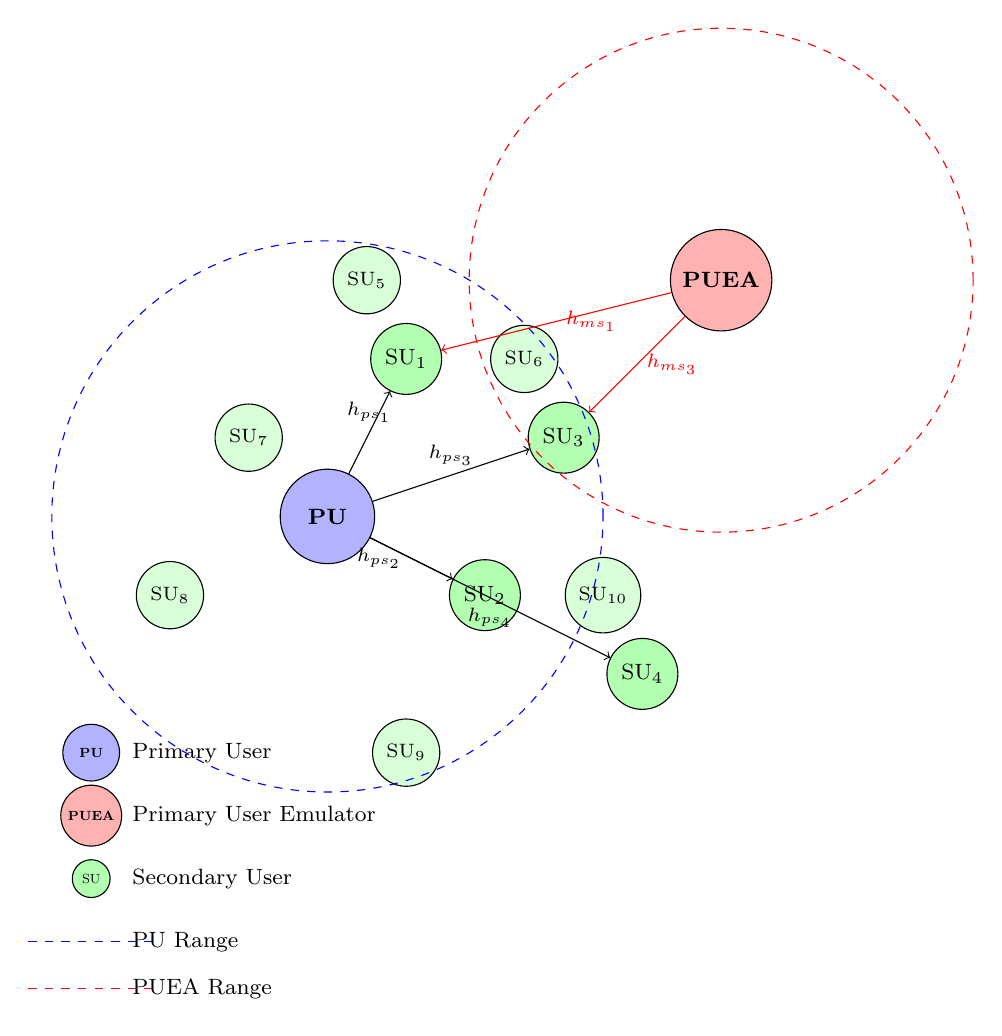
\begin{tikzpicture}[scale=1.0]
        % Define styles for nodes
        \tikzstyle{pu}=[circle,draw,fill=blue!30,minimum size=1.2cm,font=\footnotesize\bfseries]
        \tikzstyle{puea}=[circle,draw,fill=red!30,minimum size=1.2cm,font=\footnotesize\bfseries]
        \tikzstyle{su}=[circle,draw,fill=green!30,minimum size=0.8cm,font=\footnotesize]
        \tikzstyle{su_small}=[circle,draw,fill=green!15,minimum size=0.6cm,font=\scriptsize]
        
        % Primary User
        \node[pu] (pu) at (0,0) {PU};
        
        % Primary User Emulator Attacker
        \node[puea] (puea) at (5,3) {PUEA};
        
        % Secondary Users - larger ones represent sensing nodes
        \node[su] (su1) at (1,2) {SU$_1$};
        \node[su] (su2) at (2,-1) {SU$_2$};
        \node[su] (su3) at (3,1) {SU$_3$};
        \node[su] (su4) at (4,-2) {SU$_4$};
        
        % Additional secondary users (smaller)
        \node[su_small] (su5) at (0.5,3) {SU$_5$};
        \node[su_small] (su6) at (2.5,2) {SU$_6$};
        \node[su_small] (su7) at (-1,1) {SU$_7$};
        \node[su_small] (su8) at (-2,-1) {SU$_8$};
        \node[su_small] (su9) at (1,-3) {SU$_9$};
        \node[su_small] (su10) at (3.5,-1) {SU$_{10}$};
        
        % PU transmission range
        \draw[blue, dashed] (0,0) circle (3.5cm);
        
        % PUEA transmission range
        \draw[red, dashed] (5,3) circle (3.2cm);
        
        % Connections
        \draw[->] (pu) -- node[midway, above, font=\scriptsize] {$h_{ps_1}$} (su1);
        \draw[->] (pu) -- node[midway, left, font=\scriptsize] {$h_{ps_2}$} (su2);
        \draw[->] (pu) -- node[midway, above, font=\scriptsize] {$h_{ps_3}$} (su3);
        \draw[->] (pu) -- node[midway, below, font=\scriptsize] {$h_{ps_4}$} (su4);
        
        \draw[->, red] (puea) -- node[midway, right, font=\scriptsize] {$h_{ms_1}$} (su1);
        \draw[->, red] (puea) -- node[midway, right, font=\scriptsize] {$h_{ms_3}$} (su3);
        
        % Legend
        \node[pu, scale=0.6] (lpu) at (-3,-3) {PU};
        \node[right, font=\footnotesize] at (-2.6,-3) {Primary User};
        
        \node[puea, scale=0.6] (lpuea) at (-3,-3.8) {PUEA};
        \node[right, font=\footnotesize] at (-2.6,-3.8) {Primary User Emulator};
        
        \node[su, scale=0.6] (lsu) at (-3,-4.6) {SU};
        \node[right, font=\footnotesize] at (-2.6,-4.6) {Secondary User};
        
        \draw[blue, dashed] (-3.8,-5.4) -- (-2.2,-5.4);
        \node[right, font=\footnotesize] at (-2.6,-5.4) {PU Range};
        
        \draw[red, dashed] (-3.8,-6.0) -- (-2.2,-6.0);
        \node[right, font=\footnotesize] at (-2.6,-6.0) {PUEA Range};
        
    \end{tikzpicture}
    \caption{System model for cognitive radio network with PU and PUEA}
    \label{fig:system_model}
\end{figure}
